\documentclass{article}

\usepackage{geometry}
\geometry{margin=2cm}
\usepackage{graphicx}
\usepackage{hyperref}

\hypersetup{colorlinks=true, linkcolor=blue, urlcolor=blue}
\urlstyle{same}
\begin{document}
	
	\author{Aayush Arya}
	\date{(Submitted: \today)}
	\title{}
	
	\maketitle
	
	\hrule
	\begin{center}
		PHY350 Lab Report\\
		Registration No.: 11912610 \quad Section: G2903
	\end{center}
	\hrule
	
	\section*{Aim}
	To study the variation of the resistivity of a Ge sample and determine its band gap using the four-probe method.

	\section*{Methods}
	We used the VirtualLab platform for performing this experiment {\it in silico} (see Figure \ref{fig:sim}).
	
	\begin{figure}[h]
		\centering
		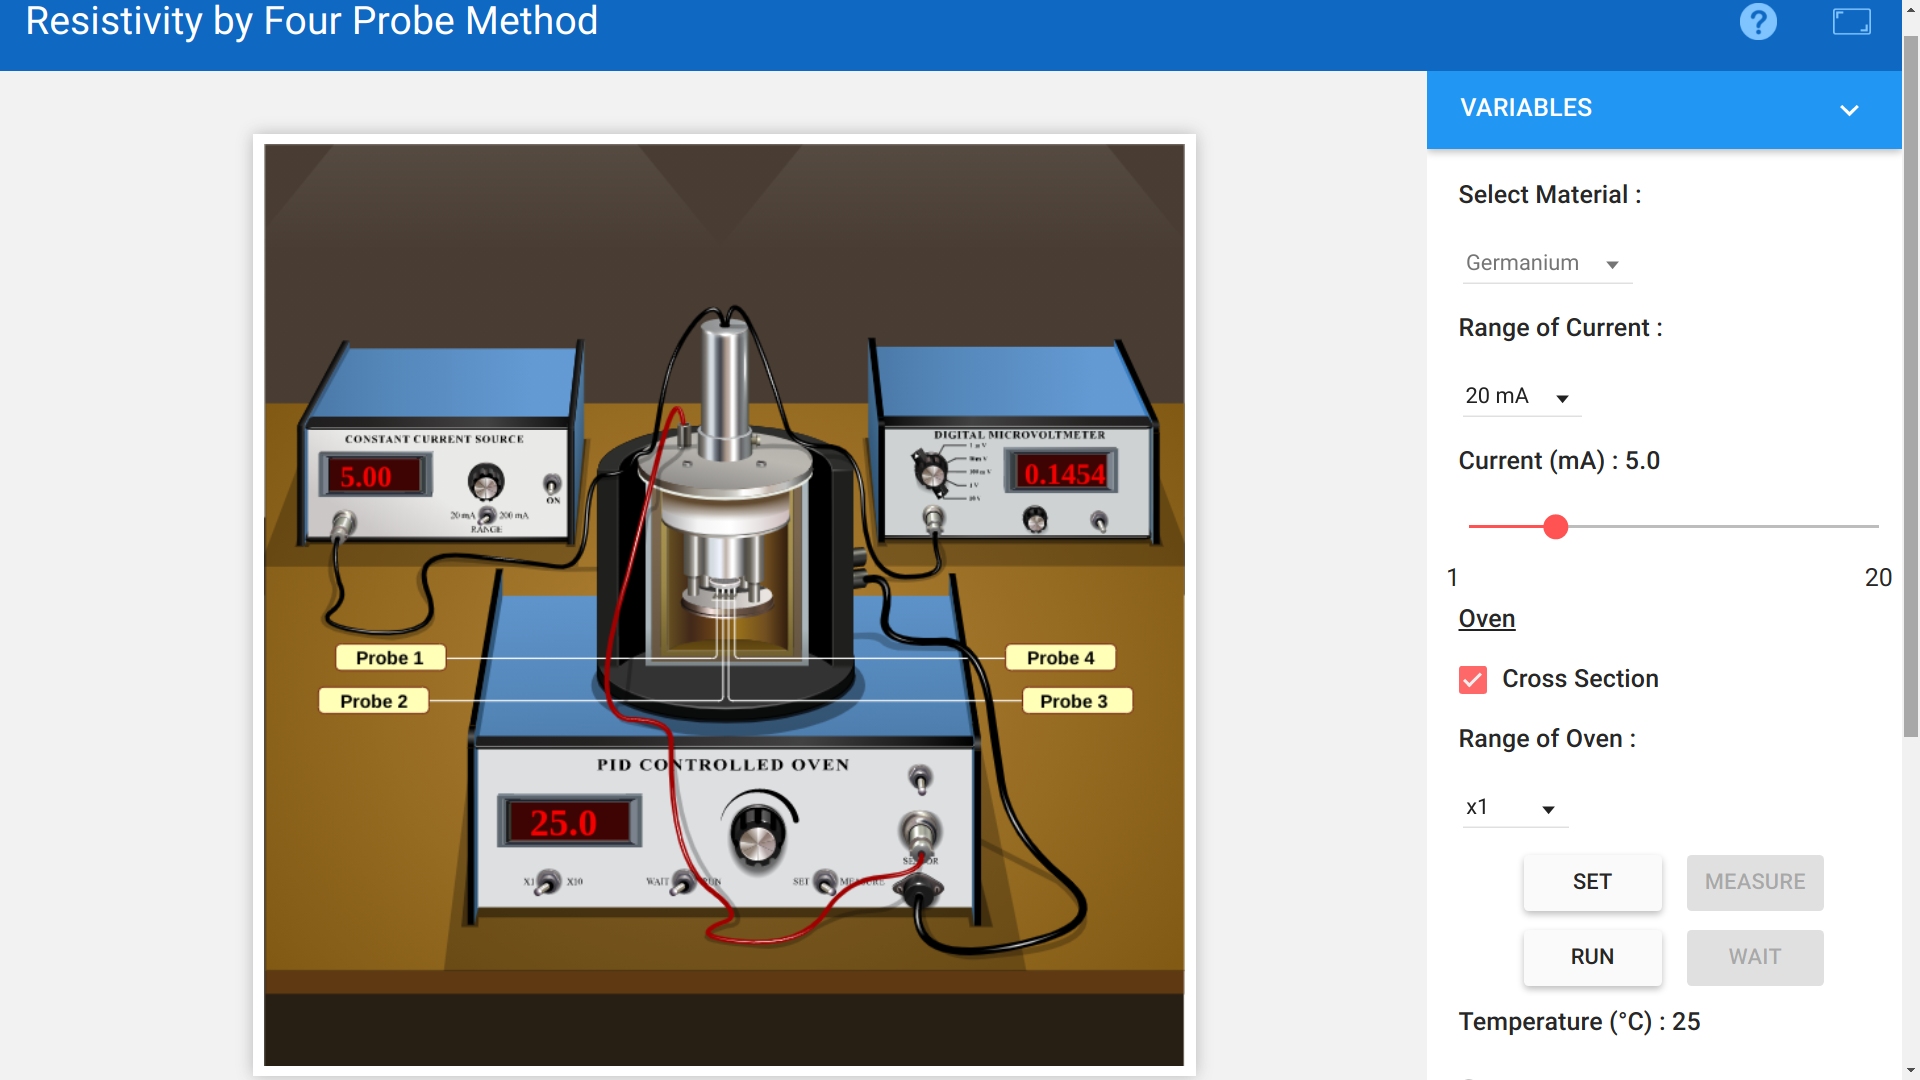
\includegraphics[width=0.8\textwidth]{four_probe_app}
		\caption{The four-probe apparatus on the VirtualLab platform of Amrita Visvavidyapeetham}
		\label{fig:sim}	
	\end{figure}

	 A Ge sample was picked from the adjustables and for different temperature values set using a PID Controlled Oven, different values of resistivity were read out directly from the platform. We report our measurements in Table \ref{meastable}.
	 
	 Since the resistivity of a semiconductor varies as
	 
	 $$ \rho = A \exp{ \left( \frac{E_g}{2kT} \right) }$$
	 
	 we can obtain the band-gap $E_g$ by finding the slope of the straight line
	 
	 $$ \log \rho = \log A + \frac{E_g}{2kT} $$
		where $k$ is the Boltzmann constant and $T$ is in Kelvins. The constant $\log A$ will determine the intercept of the plot and for our purposes, can be ignored.
		
	\section*{Results}
	\begin{table}[h]
		\centering
		\begin{tabular}{|c|c|}
			\hline
			Temperature ($^o$C) & $\rho$ (Ohm cm$^{-1}$) \\
			\hline
			25 & 6.2011  \\
			40 & 5.6819 \\
			55 & 5.2479 \\
			70 & 4.8809 \\
			85 & 4.5672 \\
			\hline
		\end{tabular}
	\caption{Measured values of resitivity ($\rho$) for different temperatures.}
	\label{meastable}
	\end{table}

	When $\log \rho$ is plotted against $1/T$
	
	\begin{figure}[h!]
		\centering
		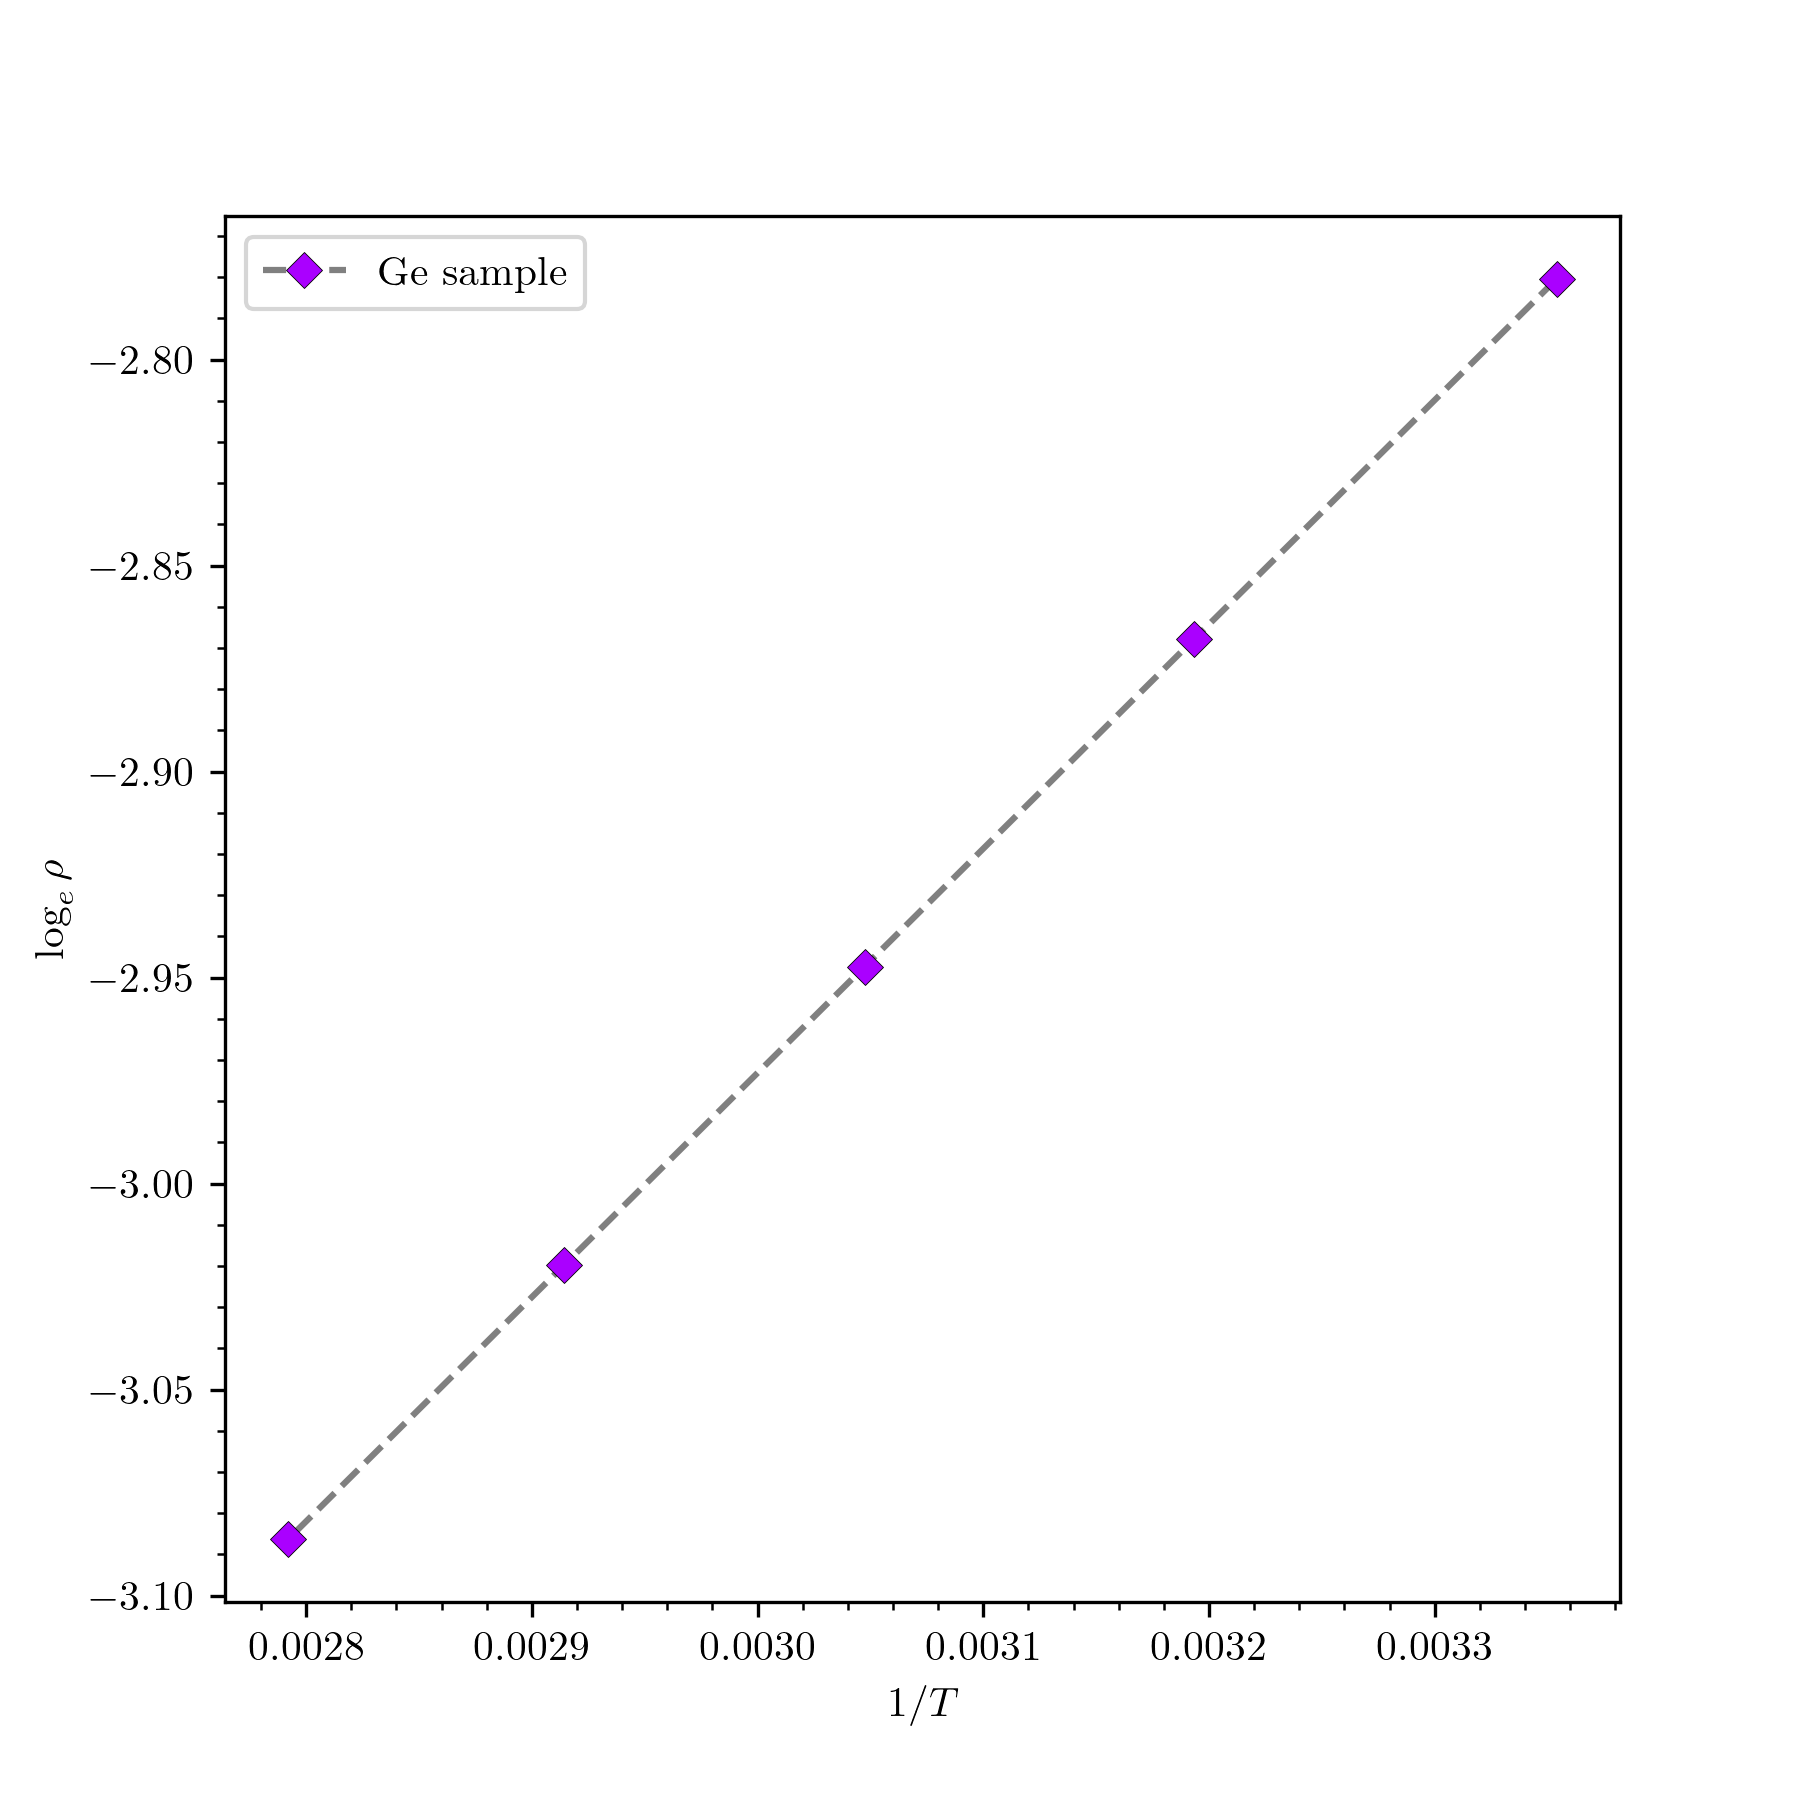
\includegraphics[width=0.6\textwidth]{temp_rho_var}
		\caption{Variation of resistivity with temperature}
		\label{fig:temp_var}
	\end{figure}

	The slope, found by a simple linear regression using the \texttt{scipy} Python package, turns out to be, $m=544.28$. Since $ m = E_g/2kT$, we get an $E_g = 2mkT$.\\
	
	which upon unit conversion gives an $E_g = 0.093$eV, not in line with the true value of around $0.67$eV.
	
	The python script used for the estimation here
\end{document}